\clearpage
\chapter{Der Industriezweig Uhr}
\section{Geschichtliches zur Uhrindustrie}
Die Schweiz ist derzeit das Land mit den meisten Uhrenexporten. Gemessen an den Exporten ist die Uhrenindustrie innerhalb der Schweiz jedoch nur die drittgrößte Industrie. Weltweit gefolgt wird die Schweiz Hongkong und China.\\ 
In den 1970er und 1980er Jahren erhielt die klassische schweizer Uhrenindustrie Konkurrenz durch die Entstehung der elektrischen Uhren und den asiatischen Markt. Nachdem sie sich bis 2015 wieder etwas erholen konnte und die Exporte von 4,3 Milliarden Franken im Jahr 1986 auf 21,5 Milliarden im Jahr 2015.\\ 
Mittlerweile schaffen es vor allem die Großmarken, sich gegen die neue Konkurrenz der Smart Watches durchzusetzen, indem sie entweder hochwertige Luxusuhren herstellen, die als Schmuckstück und Statussymbol dienen oder indem sie selbst Smart Watches entwickeln.

\section{Marktsituation}
Der reale Uhrenmarkt wird (im Gegensatz zu unserem fiktiven Uhrenmarkt) von nur wenigen Ländern beherrscht. Hong Kong, China und die Schweiz sind dabei an der Spitze. Hong Kong und China sind, wie in vielen anderen Brachen, mit Massenproduktionen die weltweit größten Uhrenproduzent. Die Uhren sind im Niedrigpreissegment angesiedelt. Hingegen ist die Schweiz mit ihren berühmten \enquote{Schweizer Uhrwerken} Weltmarktführer im hochwertigen Marktbereich. Aufgrund der hochpreisigen Uhren macht die Schweiz nur einen verschwindend geringen Anteil an der globalen Produktion aus, hingegen sie wertemäßig mit Abstand das führende Exportland ist. \\   
Die Firmen, die symbolisch für die Weltmarktführerschaft stehen, sind Swatch, Richemont und Rolex.
\\
%BILD Hersteller%
\begin{figure}[!h]
	\centering
	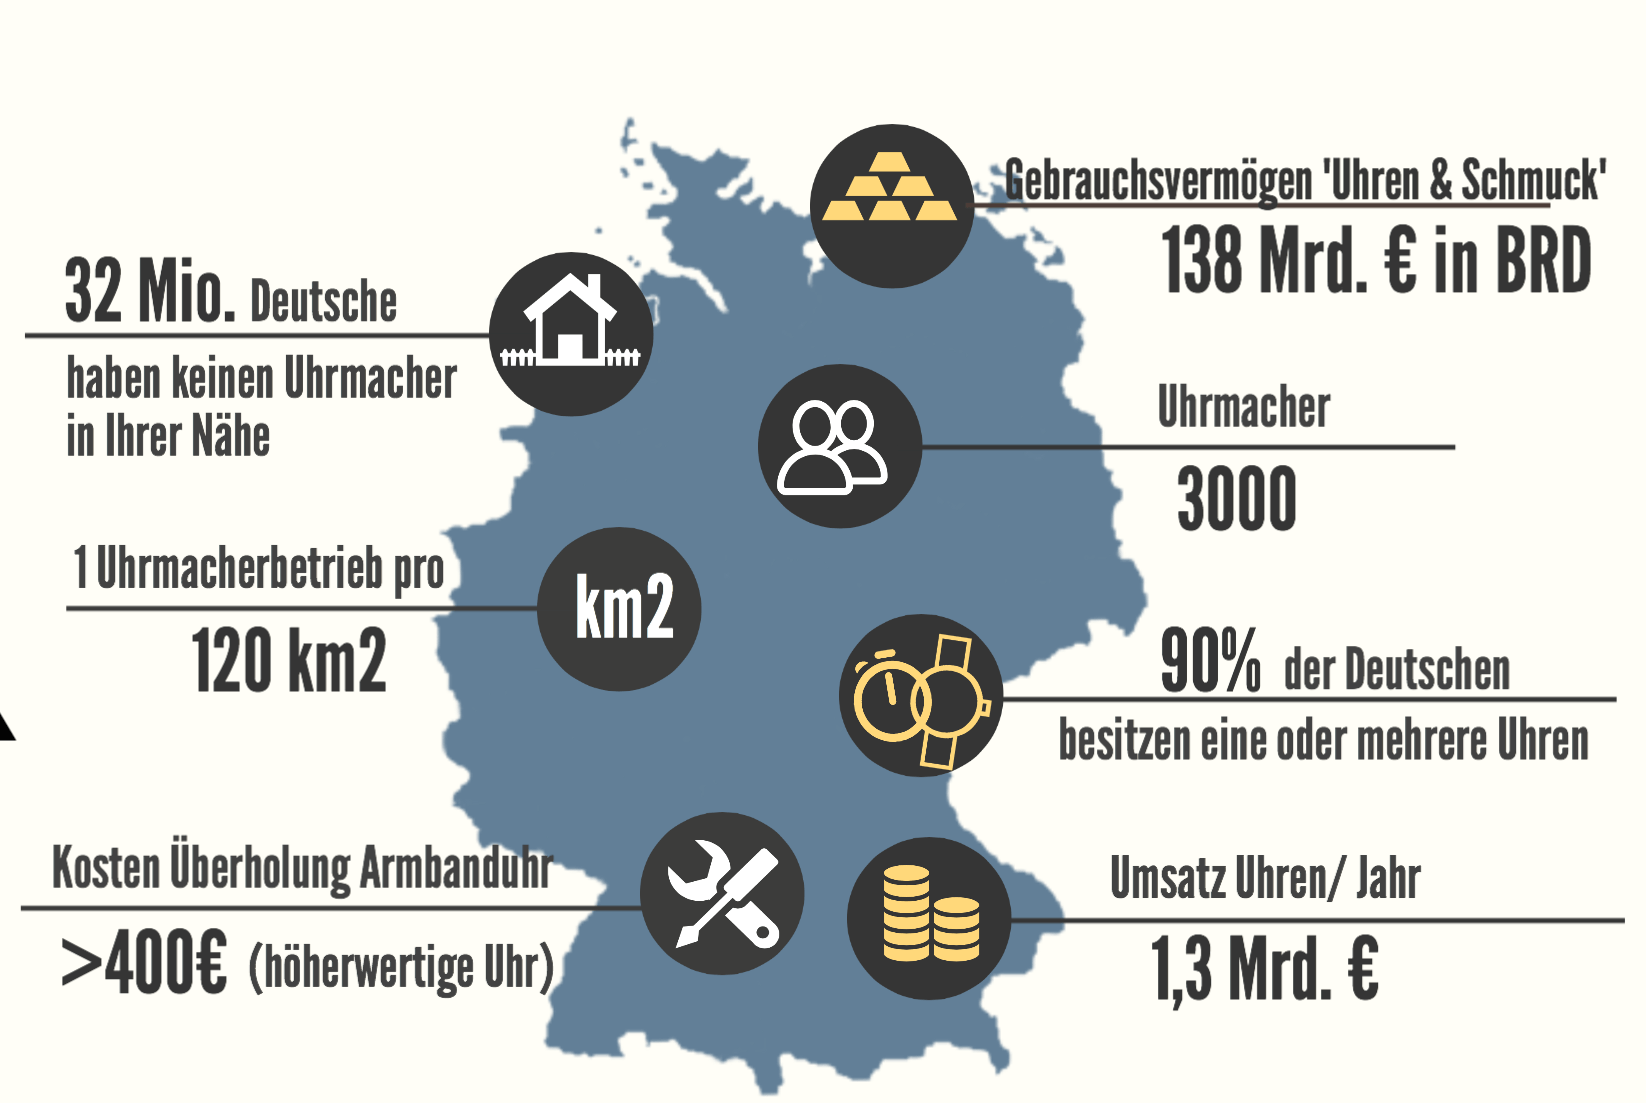
\includegraphics[scale=0.25]{statistiken/uhrenmarkt_info.png}
	\label{fig:abb1}
	\caption{Statistik: Marktanteile der führenden Uhrenhersteller} 
\end{figure} 
\\
Zusammen machen die drei Marken 40\% bis 50\% des weltweiten Uhrenumsatzes aus. Im Jahr 2016 exportierte die Schweiz Uhren im Wert von 19,8 Milliarden EURO. Gefolgt von Hong Kong (8,8) und China (5,3)
\\
%BILD Statistik EXPORT%
\begin{figure}[!h]
	\centering
	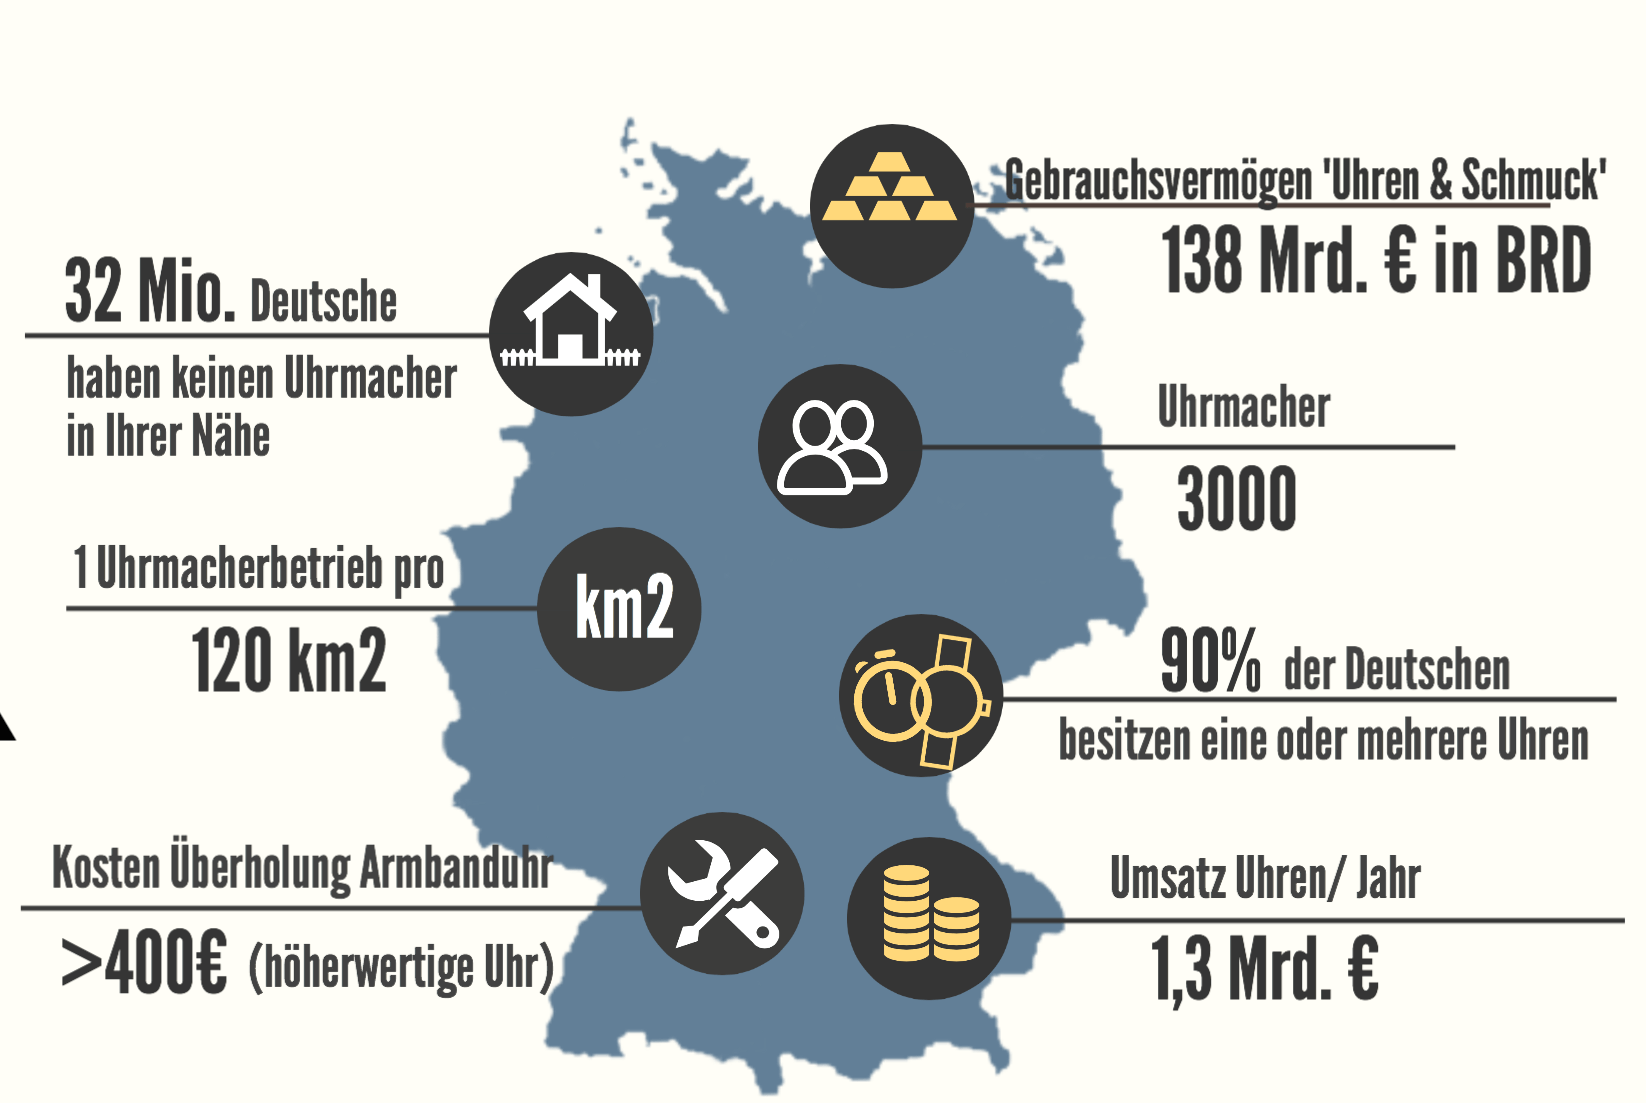
\includegraphics[scale=0.25]{statistiken/uhrenmarkt_info.png}
	\label{fig:abb1}
	\caption{Statistik: Weltweit führende Exportnationen} 
\end{figure}
\\
\begin{figure}[!h]
	\centering
	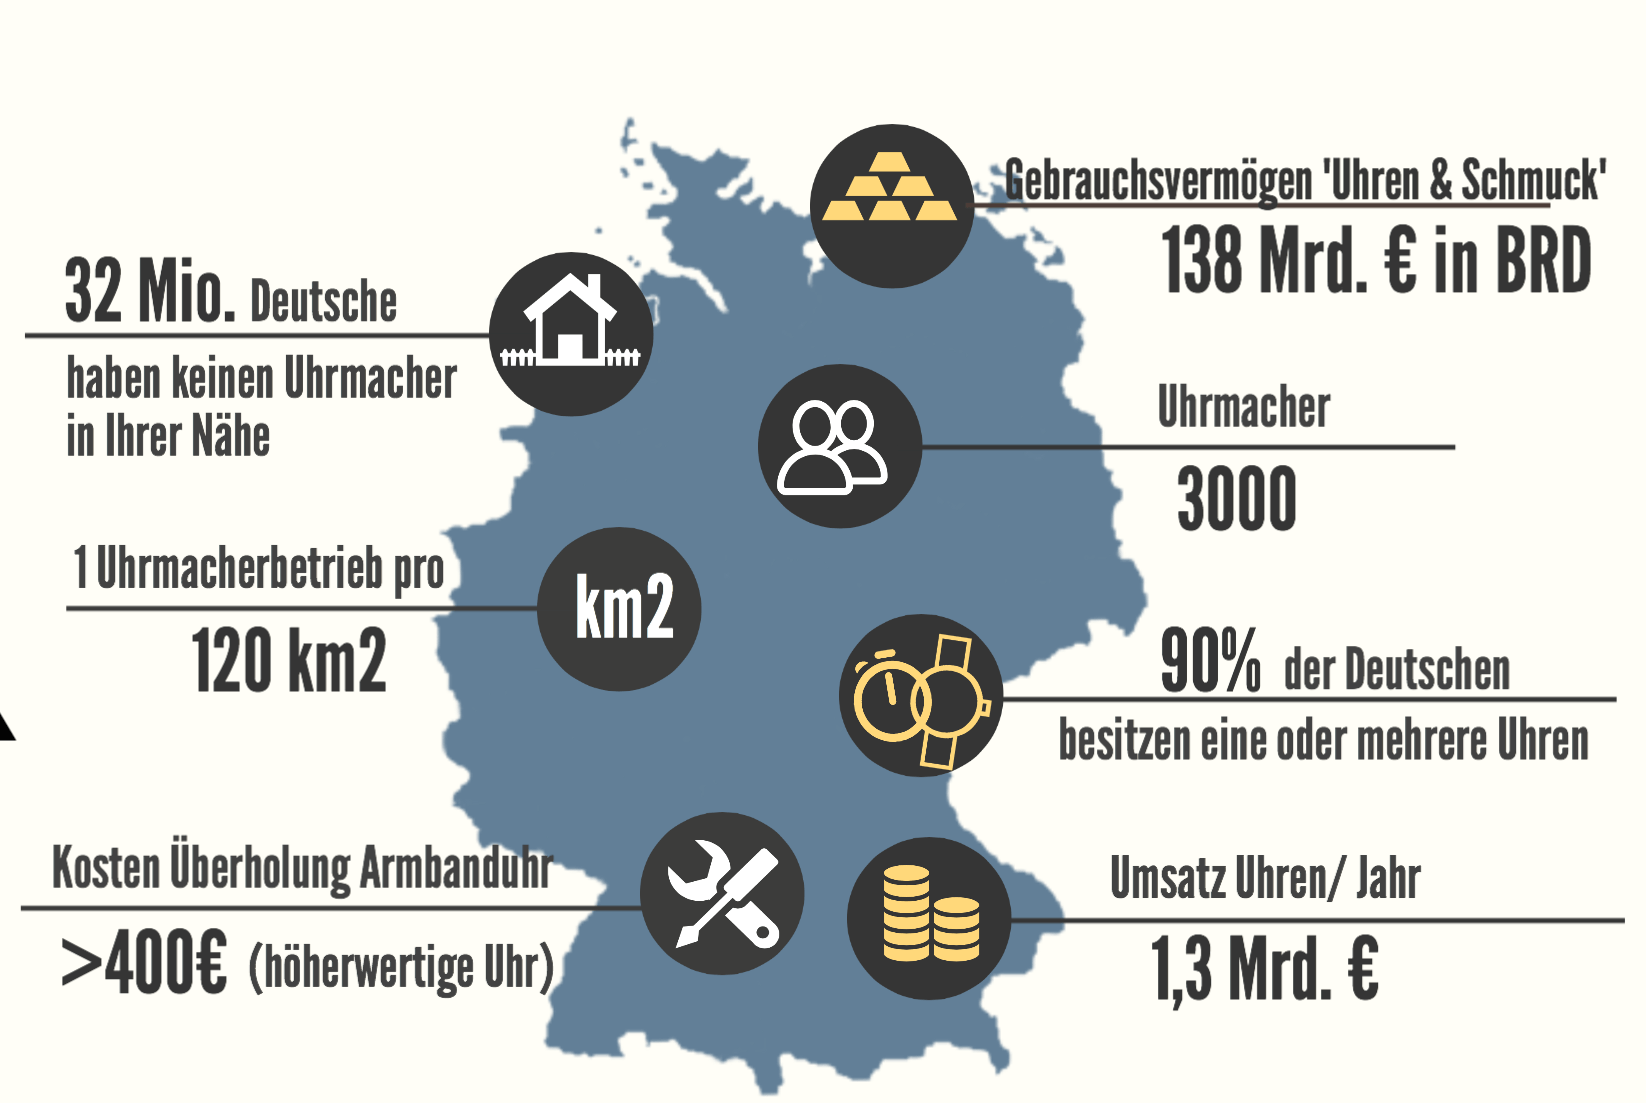
\includegraphics[scale=0.25]{statistiken/uhrenmarkt_info.png}
	\label{fig:abb1}
	\caption{Fakten zum Uhrenmarkt in Deutschland} 
\end{figure}

